
\section{Team PML 30 --${Y}$} 
	
	
        Team PML 30 -- ${Y}$ was assembled in October 2015 in Saint-Petersburg, Russia from 2 novices and 3 participants with experience, who took part in PML30 -- ${\varphi}$ and PML 30 -- ${\psi}$ teams in season 2014 - 2015. New team is based on the FTC teams that existed in our laboratory since October, 2012. 
	
	Tasks and roles of robot designing were distributed among the participants, and safety rules were established. At the first place we put spreading principles of gracious professionalism to others. All decisions were made collectively inside team with discussion to find the most optimal solutions, every idea was discussed in details to avoid missing interesting idea or making wrong decision. 
	
	During the year we took part in many events and everywhere we have tried to attract attention to our team, encourage people to take part in FTC and helped competitions organizers in the way of explaining rules and making regional qualifies as official as regional finals. Also we pursued and distributed the principles of gracious professionalism. Talking to the press, we hoped to attract more attention to our team and to the competition in general, as well as attracting sponsors. The latter was important because of the need for funds - purchasing materials and equipment costs a lot.
	
	The team took part in the three qualifying competitions and in the regional finals. We have met number of team there and share our experience with them. Aside from meeting new teams we also kept in touch through Facebook with teams we met during previous years: Stuy Fission 310 from USA who we met in Sochi last year, a team from Romania, Auto Vortex who we met on regional finals the same season. Also, there is an active group chat with a large number of Russian teams. You can find the team page in Facebook at the address https://www.facebook.com/pages/FTC-team-PML30-PHI.
	To increase the efficiency of our team work we used the version control system GitHub, which allows the entire team to work simultaneously on a single projects without losing files and providing easy way to resolve problems. Also for writing technical books we had used professional typesetting system LaTeX.
	
	For our team spreading information about FTC is very important and we try to motivate to take part in it as much people, as possible. We consider FTC very useful and interesting competitions, so we are very happy to participate in it. 
	\begin{figure}[H]
		\center{\includegraphics[scale=0.2]{1Introduction/2Our_team/images/09}}\\
	\end{figure}
\fillpage

\subsubsection{Instructors}

\begin{figure}[H]
	
	\begin{minipage}[h]{0.47\linewidth}
		Luzin Dmitry\\
		\emph{Head of Robotics Department in Phys-Math Lyceum 30, Saint-Peterburg, Russia. Main coach of FTC team.\\}
		\emph{Information: 25 years old, in robotics 5 years, in FTC 3 years.}
	\end{minipage}
	\hfill
	\begin{minipage}{0.47\linewidth}
		\center{\includegraphics[scale=0.3]{1Introduction/2Our_team/images/07}}\\
	\end{minipage}
	\vfill
	\begin{minipage}[h]{0.47\linewidth}
		\center{\includegraphics[scale=0.35]{1Introduction/2Our_team/images/08}}\\
	\end{minipage}
	\hfill
	\begin{minipage}{0.47\linewidth}
		Luzina Ekaterina \\
		\emph{Professor of Robotics Department in Phys-Math Lyceum 30, Saint-Peterburg, Russia. Tutor of FTC team. \\}
		\emph{Information: 25 years old, in robotics 5 years, in FTC 3 years.}
	\end{minipage}
\end{figure}

\begin{figure}[H]
	\begin{minipage}[h]{0.47\linewidth}
		\center{\includegraphics[scale=0.25]{1Introduction/2Our_team/images/05}}\\
	\end{minipage}
	\hfill
	\begin{minipage}{0.47\linewidth}
		Fedotov Anton \\ 
		\emph{Professor of Robotics Department in Phys-Math Lyceum 30, Saint-Peterburg, Russia. Tutor of FTC team. \\}
		\emph{Information: 22 years old, in robotics 4 years, in FTC 3 years.}
	\end{minipage}	
	\vfill 
\end{figure}

\begin{figure}[H]
	\begin{minipage}{0.47\linewidth}
		Krylov Georgii \\ 
		\emph{Professor of Robotics Department in Phys-Math Lyceum 30, Saint-Peterburg, Russia. Tutor of FTC team. \\}
		\emph{Information: 18 years old, in robotics 4 years, in FTC 4 years.}
	\end{minipage}	
	\hfill
	\begin{minipage}[h]{0.47\linewidth}
		\center{\includegraphics[scale=0.11]{1Introduction/2Our_team/images/06}}\\
	\end{minipage}
	\vfill 
\end{figure}

\fillpage

\subsubsection{Team members}

\begin{figure}[H]
	\begin{minipage}{0.47\linewidth}
		Nikita Safronov\\
		\emph{Role in team: captain, reserve drive-operator, responsible for writing the technical book, responsible for elevator and winch.\\}
		\emph{Information: 17 years old, in robotics 4 years, in FTC 2 years.\\} 
		\emph{Why I chose FTC: "I have chosen FIRST because I enjoy working with mechanisms and finding unusual technical decisions for solving problems. Also working on this project helps me to get new skills in a sphere of engineering. In this case I know, that I don't spend my time in vain."}				
	\end{minipage}
	\hfill
	\begin{minipage}{0.47\linewidth}
		\center{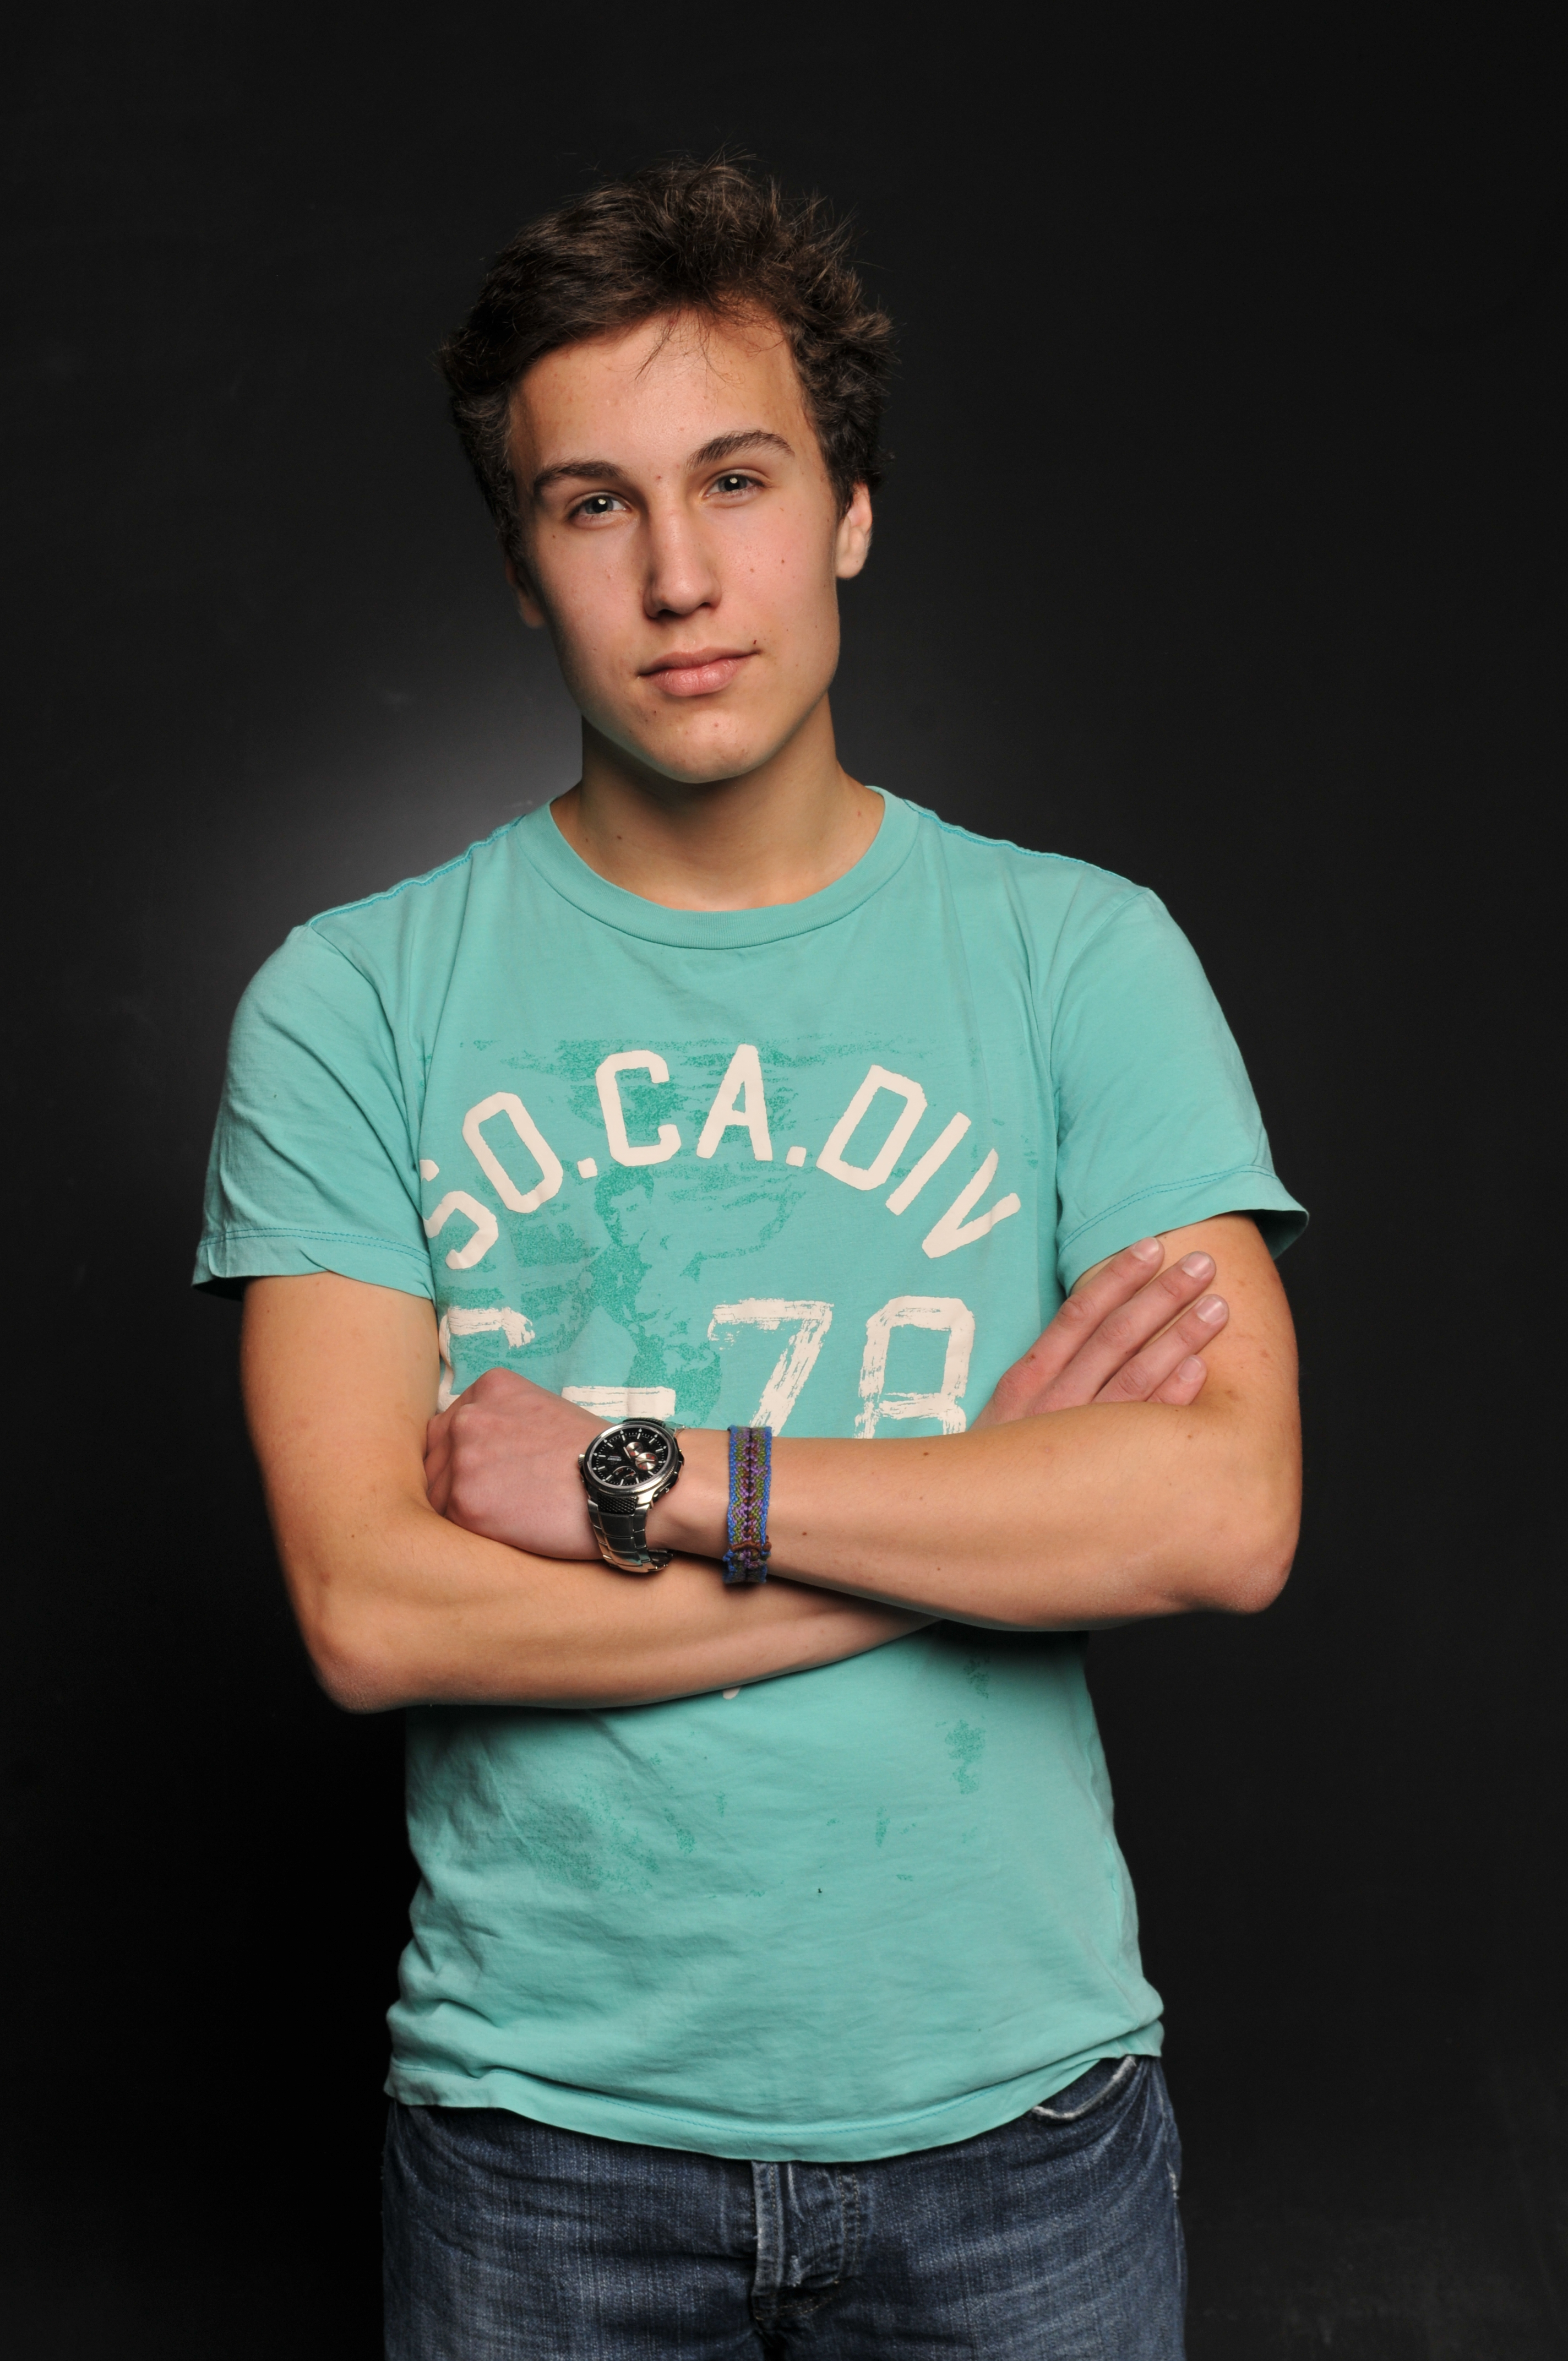
\includegraphics[scale=0.22]{1Introduction/2Our_team/images/03}}\\
	\end{minipage}
\end{figure}

\begin{figure}[H]
	\begin{minipage}[h]{0.47\linewidth}
		\center{\includegraphics[scale=0.50]{1Introduction/2Our_team/images/10}}\\
	\end{minipage}
	\hfill
	\begin{minipage}[h]{0.47\linewidth}
		Alexandr Iliasov \\
		\emph{Role in team: operator-2, decorating robot, Power Design, responsible for the bucket.\\}
		\emph{Information: 16 years old, in robotics 3 years, in FTC 2 year. \\}
		\emph{Why I chose FTC: "I choose to partipucate in the FTC, because it requiers many skills in a lot of interesting themes: physics, engineering, programming, geometry. Also, you need to work in team, argument your choise and listen others. You need find problems and solve it. All that skills you can obtain in FTC."}		
	\end{minipage}
	\vfill
\end{figure}

\begin{figure}[H]
	\begin{minipage}[h]{0.47\linewidth}
	    Anton Ponikarovsky\\
		\emph{Role in team: , communication with other teams and community, reserve operator-2, responsible. \\  }
		\emph{Information: 17 years old, in robotics 3 years, in FTC 2 year. \\}
		\emph{Why I chose FTC: "I decided to join FTC because I believe that this competition is one of the most challenging of those, which are familiar to me. It requires responsibility, capability of working in team, communication with other teams, working on hardware, software and even tecnical documentation. All the experience you accumulate through doing FTC, you can apply in your future profession, if it is technical oriented."}			
	\end{minipage}
	\hfill
	\begin{minipage}[h]{0.47\linewidth}
		\center{\includegraphics[scale=0.3]{1Introduction/2Our_team/images/12}}\\
	\end{minipage}
\end{figure}

\begin{figure}[H]
	\begin{minipage}{0.47\linewidth}
		\center{\includegraphics[scale=0.22]{1Introduction/2Our_team/images/01}}\\
	\end{minipage}
	\hfill
	\begin{minipage}{0.47\linewidth}
		Andrew Nemow\\
		\emph{Role in team: drive-operator, responsible for the writing the program, responsible for debris collecting systems.\\}
		\emph{Information: 16 years old, in robotics 2 years, in FTC 1 years.\\} 
		\emph{Why I chose FTC: "When I first I attended the event FTC saw hefty metal robots, with enthusiasm and without hesitation decided that I would like to do this."}				
	\end{minipage}
	\vfill
\end{figure}

\begin{figure}[H]
	\begin{minipage}{0.47\linewidth}
		Gordei Kravzov\\
		\emph{Role in team: development strategy in the game, responsible for chassis.\\ }
		\emph{Information: 16 years old, in robotics 2 years, in FTC 1 year. \\ } 
		\emph{Why I chose FTC:"I enjoy making huge and complicated mechanisms work, that's why I chose FIRST FTC. In my opinion it's a great way to improve your skills and broaden the mind doing something that you love by the whole heart."}		
	\end{minipage}
	\hfill
	\begin{minipage}[h]{0.47\linewidth}
		\center{\includegraphics[scale=0.25]{1Introduction/2Our_team/images/11}}\\
	\end{minipage}
\end{figure}

\fillpage


